\documentclass[]{beamer}
\usetheme{Dresden}
% \useoutertheme{split}

\usepackage{color}
\usepackage{graphicx}
\usepackage{listings}
\usepackage{lmodern} %% allow bold keywords
\usepackage{menukeys}
\usepackage{qtree}

\definecolor{darkgreen}{rgb}{0,0.5,0}
\definecolor{lightblue}{rgb}{0.2,0.2,1}

\lstset{language=Java,
	basicstyle=\ttfamily\footnotesize,
	keywordstyle=\color{purple},
	commentstyle=\color{darkgreen},
	numberstyle=\tiny\color{gray},
	stringstyle=\color{blue},
	tabsize=4,
	showstringspaces=false,
	breaklines=true,
	keepspaces=true,
	numbers=left,
	escapechar=@
}
\usepackage{multicol}

\title{IO}
\subtitle{Input/Output}
\author{Nico Westerbeck}
\date{\today}


\begin{document}

\titlepage

\begin{frame}{Introduction}
What we learned until now:
\begin{itemize}
	\item Thinking in code
	\begin{itemize}
		\item Primitive Types
		\item Usage of Eclipse
		\item Arrays
		\item Collections
		\item Exceptions
	\end{itemize}
	\item Thinking in objects
	\begin{itemize}
		\item Transferring a task into a class-structure
		\item Declaring classes in java
		\item Inheritance
		\item Abstract classes / interfaces
	\end{itemize}
	\item Usage of Fredo's Simple-GUI
\end{itemize}

\end{frame}

\begin{frame}{Today}
	\begin{itemize}
		\item IO
		\item Enums
		\item Whatever =)
	\end{itemize}
\end{frame}


\begin{frame}{IO}
	\begin{center}
		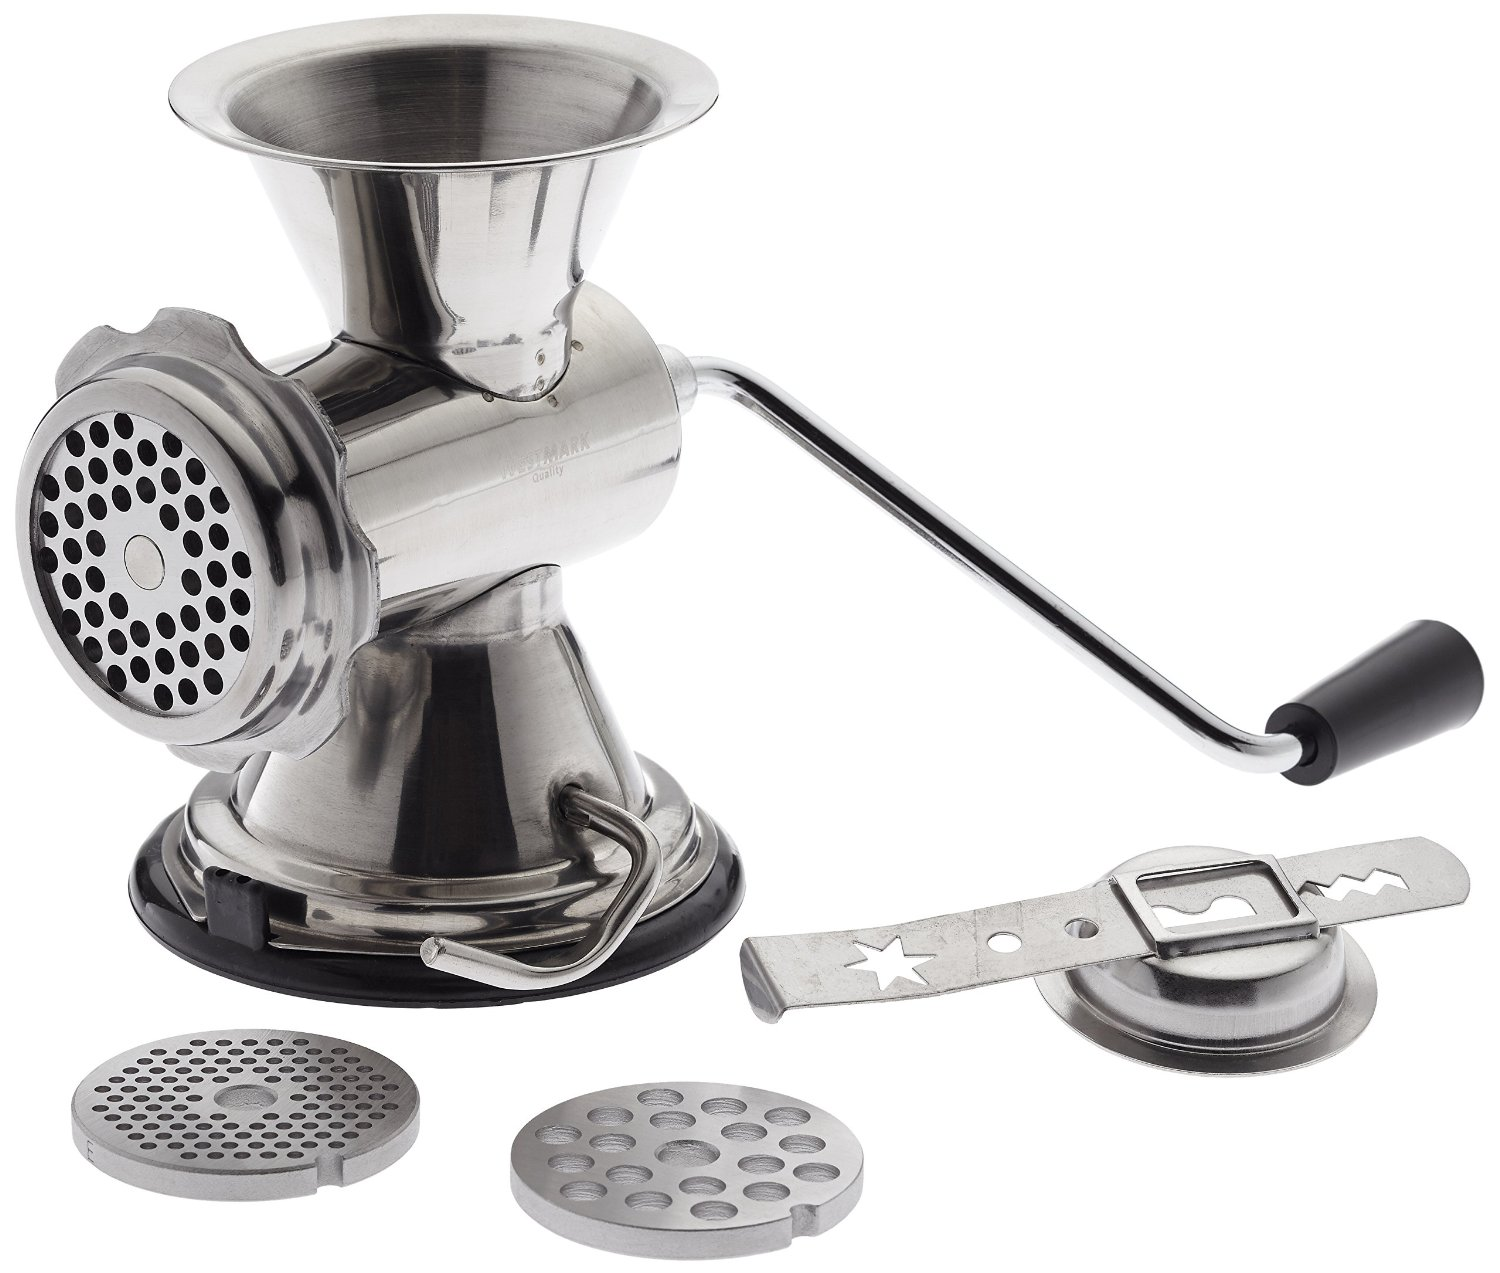
\includegraphics[width=8cm]{res/cookiepress.jpg}
	\end{center}
	% Cookiepress is metaphorfor stream, stream is the piece of metal at the end
	% Cookies are data
	% The machine is driven by some raw source
\end{frame}

\begin{frame}{IO}
	\begin{center}
		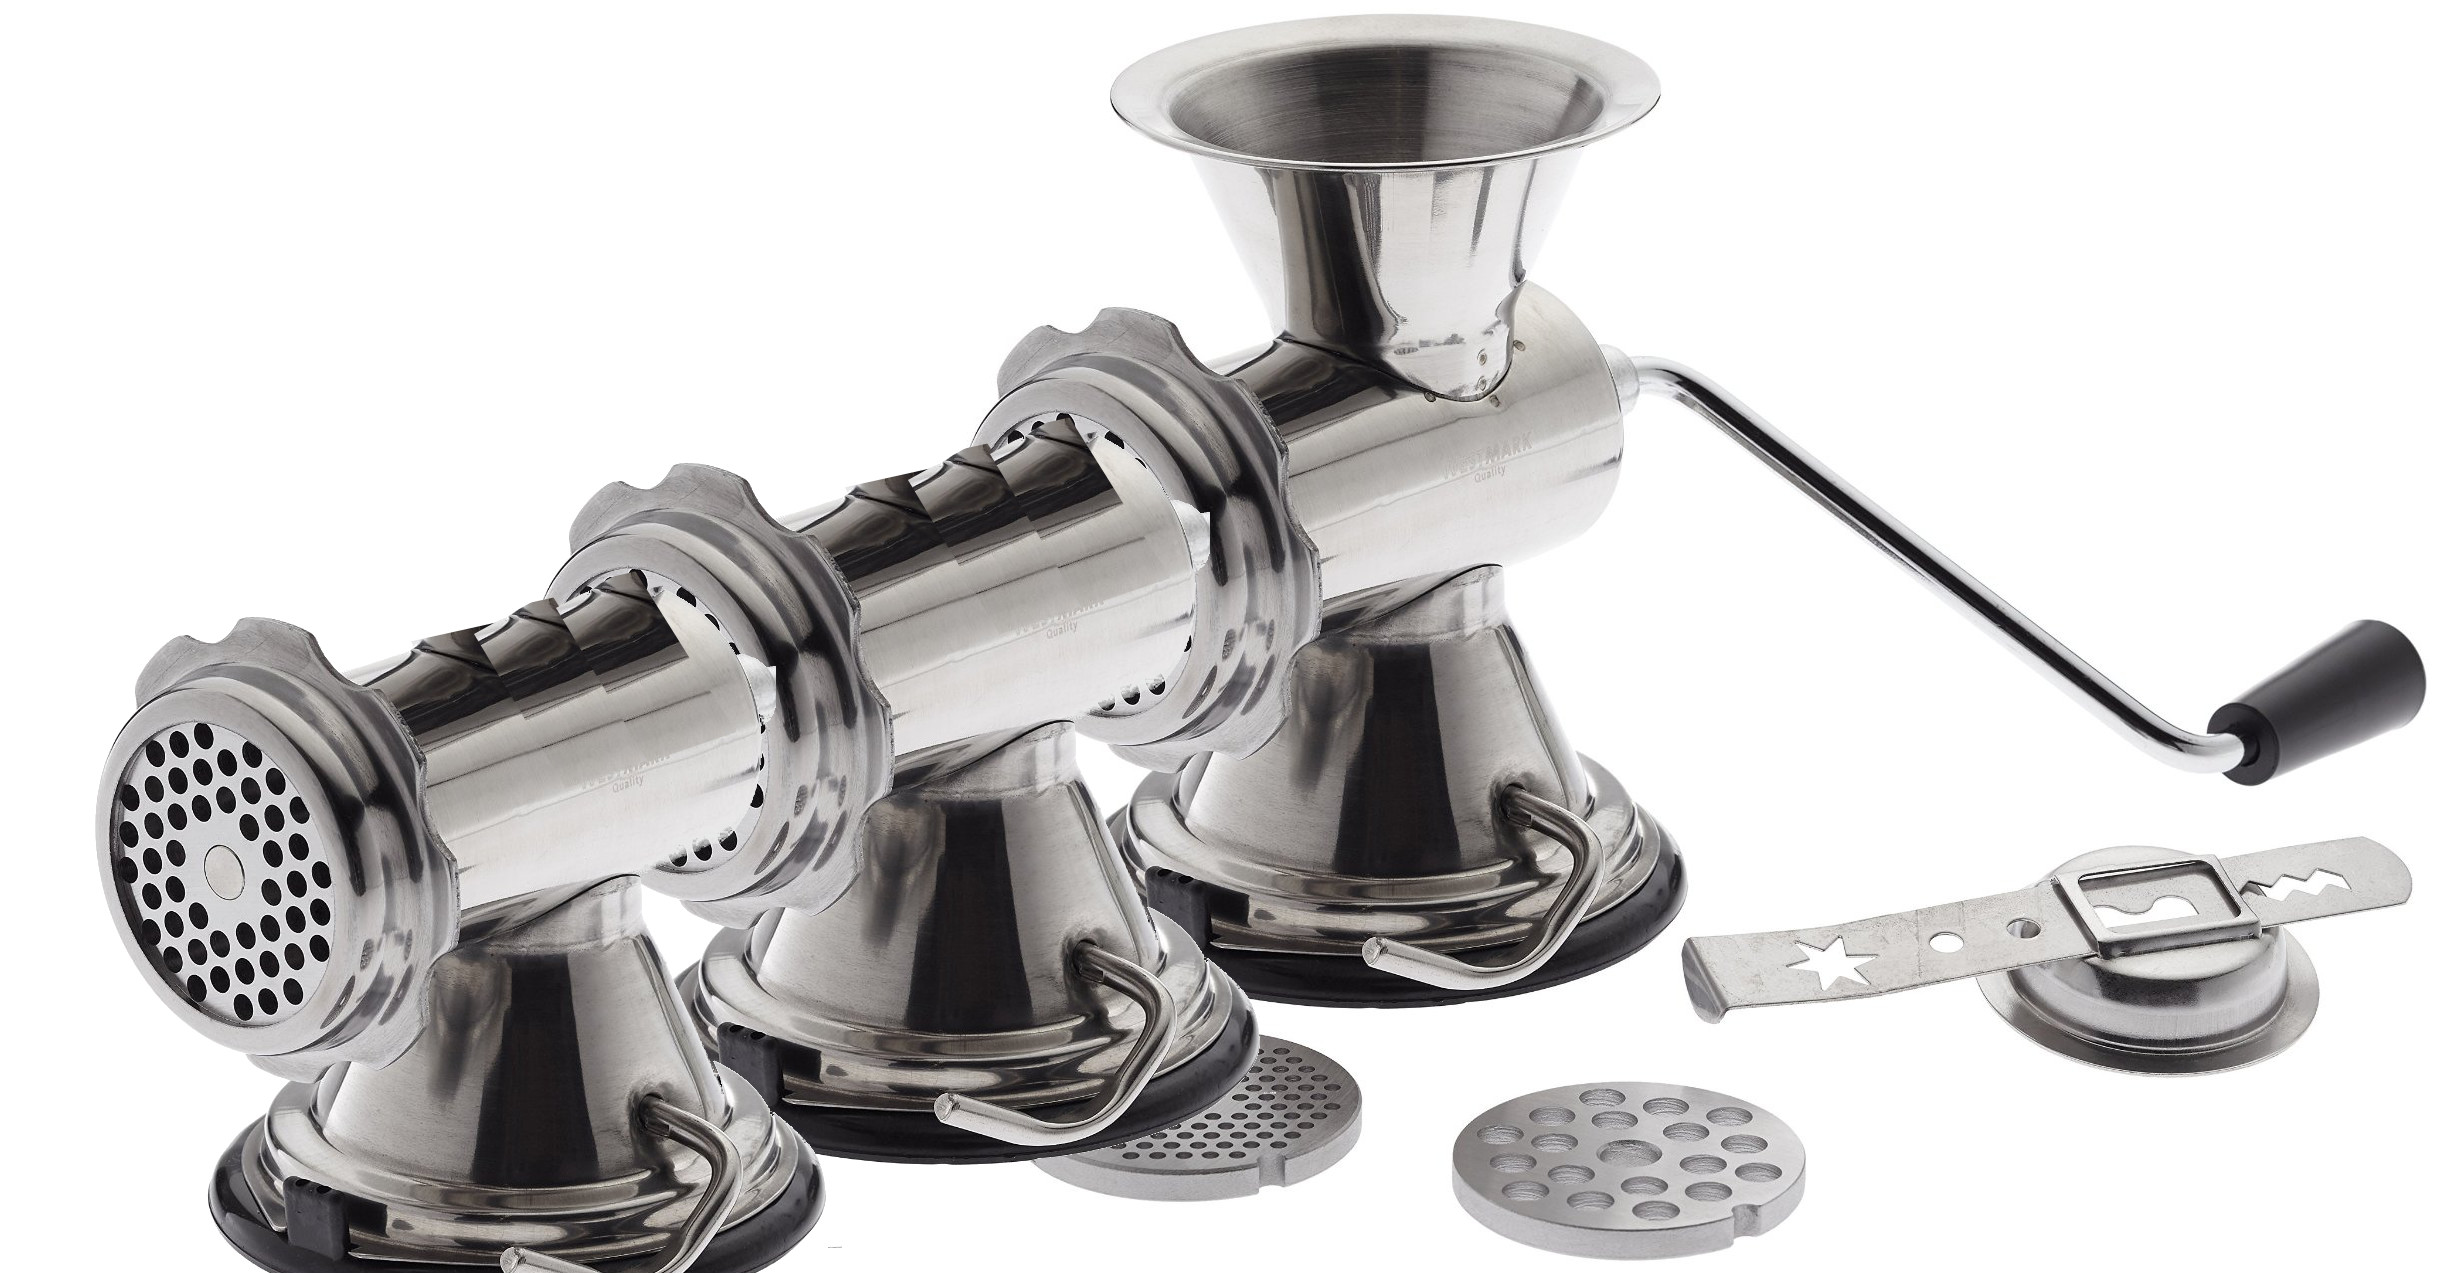
\includegraphics[width=10cm]{res/cookiepress2.jpg}
	\end{center}
	% Streams can be combined
	% Ask them how they may have designed this (INHERITAAAAANCEEE!!!!)
\end{frame}

\begin{frame}{Purposes}
	\begin{itemize}
		\item Reading/Writing files
		\item Network communication
		\item Encryption
		\item Compression
		\item Buffering
		\item Encoding
	\end{itemize}
\end{frame}

\begin{frame}{Basic streams}
	\begin{multicols}{2}
	InputStream\\
	\begin{itemize}
		\item Basic method: \\ int read() - Read a byte
		\item Reading purposes
		\item Some implementing Classes
		\begin{itemize}
			\item AudioInputStream
			\item ByteArrayInputStream
			\item \emph{FileInputStream}
		\end{itemize}
	\end{itemize}
	\columnbreak
	OutputStream\\
	\begin{itemize}
		\item Basic method: \\ write(int b) - Write a byte
		\item Writing purposes *.*
		\item Some implementing Classes
		\begin{itemize}
			\item \emph{FileOutputStream}
			\item FilterOutputStream
			\item ObjectOutputStream
		\end{itemize}
	\end{itemize}
	\end{multicols}
\end{frame}

% Because it would not be complicated enough, java introduced Readers

\begin{frame}{Basic character streams}
	\begin{multicols}{2}
	Reader\
	\begin{itemize}
		\item Basic method: \\ int read() - Read a char
		\item Text reading purposes
		\item Some implementing Classes
		\begin{itemize}
			\item \emph{BufferedReader}
			\item CharArrayReader
			\item FilterReader
		\end{itemize}
	\end{itemize}
	\columnbreak
	Writer\\
	\begin{itemize}
		\item Basic method: \\ write(int b) - Write a char
		\item Text writing purposes
		\item Some implementing Classes
		\begin{itemize}
			\item \emph{BufferedWriter}
			\item CharArrayWriter
			\item FilterWriter
		\end{itemize}
		\only<2-2>{\item And: write(String s) - Write a String}
	\end{itemize}
	\end{multicols}
\end{frame}

\begin{frame}{File-Streams}
	Benutzung in Eclipse...
\end{frame}

\begin{frame}{Enumerations}
	
\end{frame}

\begin{frame}[fragile]{Enumerations}
\begin{lstlisting}
public enum Colors {
	RED,
	GREEN,
	BLUE;
}
// ...
Colors myColor = Colors.RED;
\end{lstlisting}
\end{frame}

\begin{frame}[fragile]{Enumerations}
\begin{lstlisting}
System.out.println(Colors.RED.name());
System.out.println(Colors.RED.ordinal());
\end{lstlisting}
% Let them guess the effect of these methods
% Outline parallel to classes...
\end{frame}

\begin{frame}[fragile]{Enumerations}
\begin{lstlisting}
public enum Colors {
	RED(255, 0, 0),
	GREEN(0, 255, 0),
	BLUE(0, 0, 255);
	
	private int r, g, b;
	private Colors(int r, int g, int b) {
		this.r = r;
		this.g = g;
		this.b = b;
	}
	
	public String getRGB() {
		return "R:" + r + " G:" + g + " B:" + b;
	}
}
\end{lstlisting}
\end{frame}

\end{document}